\documentclass[]{scrartcl}
\usepackage{lmodern}
\usepackage{amssymb,amsmath}
\usepackage{ifxetex,ifluatex}
\usepackage{fixltx2e} % provides \textsubscript
\ifnum 0\ifxetex 1\fi\ifluatex 1\fi=0 % if pdftex
  \usepackage[T1]{fontenc}
  \usepackage[utf8]{inputenc}
\else % if luatex or xelatex
  \ifxetex
    \usepackage{mathspec}
  \else
    \usepackage{fontspec}
  \fi
  \defaultfontfeatures{Ligatures=TeX,Scale=MatchLowercase}
\fi
% use upquote if available, for straight quotes in verbatim environments
\IfFileExists{upquote.sty}{\usepackage{upquote}}{}
% use microtype if available
\IfFileExists{microtype.sty}{%
\usepackage{microtype}
\UseMicrotypeSet[protrusion]{basicmath} % disable protrusion for tt fonts
}{}
\usepackage{hyperref}
\hypersetup{unicode=true,
            pdftitle={Angabe},
            pdfauthor={Team\ldots{}},
            pdfborder={0 0 0},
            breaklinks=true}
\urlstyle{same}  % don't use monospace font for urls
\IfFileExists{parskip.sty}{%
\usepackage{parskip}
}{% else
\setlength{\parindent}{0pt}
\setlength{\parskip}{6pt plus 2pt minus 1pt}
}
\setlength{\emergencystretch}{3em}  % prevent overfull lines
\providecommand{\tightlist}{%
  \setlength{\itemsep}{0pt}\setlength{\parskip}{0pt}}
\setcounter{secnumdepth}{5}
% Redefines (sub)paragraphs to behave more like sections
\ifx\paragraph\undefined\else
\let\oldparagraph\paragraph
\renewcommand{\paragraph}[1]{\oldparagraph{#1}\mbox{}}
\fi
\ifx\subparagraph\undefined\else
\let\oldsubparagraph\subparagraph
\renewcommand{\subparagraph}[1]{\oldsubparagraph{#1}\mbox{}}
\fi

\usepackage{graphicx}
\usepackage{array}
\usepackage{ragged2e}
\usepackage[section]{placeins}
\makeatletter
\AtBeginDocument{%
  \expandafter\renewcommand\expandafter\subsection\expandafter{%
    \expandafter\@fb@secFB\subsection
  }%
}
\makeatother

\title{Modell eines Insel-Callshops}
\providecommand{\subtitle}[1]{}
\subtitle{2. Projekt zu Modellierung und Simulation}
\author{Daniel Graf, Dimitrie Diez, Arne Schöntag, Peter Müller}
\date{}

\begin{document}

\maketitle

\tableofcontents
\section{Einführung}
Simulationen haben in der moderne einen sehr hohen Stellenwert erlangt, da durch sie zahlreiche, oftmals sehr genaue, Zukunftsprognosen erstellt werden können. Als Grundlage für die Simulationen dienen in der Regel Modelle, welche einen Ausschnitt der Wirklichkeit abbilden. Das Thema dieser Studienarbeit ist die Simulation eines Callshops, bzw. des Telefons in einem Callshop, in einem Inseldorf. Dieser wird für günstige Telefonate ins Ausland verwendet. 

\section{Beschreibung des Modells}
Für die Simulation des Insel-Callshops wird ein Warteschlagenmodell mit Clients und zunächst nur einem Server verwendet. Jede Person die den CallShop betritt wird durch einen neuen Client repräsentiert. Das Telefon des Shops ist durch den Server dargestellt. Möchte eine Person das Telefon zu einem Zeitpunkt benützen, zu dem bereits eine andere Person telefoniert, muss sie sich hinten anstellen und warten, bis die Person ihr Telefonat beendet hat. Im Modell wird dieses durch eine Warteschlage (Queue) realisiert, in die sich ankommende Clients einordnen und sobald der Server nichtmehr belegt ist nach dem FIFO (first in first out) Prinzip bedient werden. 

Im Modell werden sowohl die Ankunftszeiten der Clients, als auch die Dauer der Telefonate durch eine negative Exponentialverteilung beschrieben, da diese sehr nah an den real beoachteten Verhalten liegt. Der mathematische Hintergrund liegt in der Eigenschaft der Exponentialfunktion zugrunde. Die Exponentialverteilung ist die einzige kontinuierliche Verteilung, welche zugleich die Markoveigenschaft, die sogenannte Gedächtnislosigkeit, erfüllt. Diese besagt, dass die seit dem letzten Ereignis vergangene Zeit (in diesem Beispiel Anrufer) keinen Einfluss auf die Verteilung der Zeit bis zum nächsten Ereignis (bis zum nächsten Anruf) hat. 
Quelle: http://www.mathepedia.de/Exponentialverteilung.aspx

Darüber hinaus wird ein zweites Modell betrachtet, in welchem die Bewohner des Inseldorfes (Einheimische) bevorzugt werden. Im weiteren Verlauf der Studienarbeit werden diese mit VIP bezeichnet. Der grundlegende Ablauf verläuft wie beim ersten Modell. Allerdings wird, bevor der nächste Client (FIFO Prinzip) telefonieren darf, die Queue nach einem VIP durchsucht. Befindet sich ein VIP in der Queue, wird dieser bevorzugt und darf zuerst telfonieren. 

In einem dritten Modell befindet sich ein weiteres Telefon im Callshop. Von den nun zwei Telefonen (zwei Server), behandelt eines alle ankommenden Personen (Clients) gleichberechtigt (analog zum ersten Modell). Das zweite Telefon bevorzugt die VIPs und behandelt andere Personen nur, wenn kein VIP wartet (analog zum zweiten Modell).

\section{Anforderungen/Requirements}

\section{Softwaredesign}

\section{Überprüfung auf Exponentialverteilung}
Im Zuge dieses Kapitels erfolgt die Überprüfung der, im Zuge der implementierten Simulation, generierten Zufallszahlen. Diese sollen, wie in den Anforderungen definiert, negativ exponentialverteilt sein. \\
Die Überprüfung erfolgt zunächst graphisch mittels eines Histogramms und eines Qunatil-Quantil-Plots. Im Anschluss erfolgt die rechnerische Überprüfung mittels Shapiro-Wilk-, Cramér-von-Mises- und Anderson-Darling-Test.

\subsection{Graphische Überprüfung}
\begin{figure}[!htb]
	\centering
	\begin{minipage}{.5\textwidth}
		\centering
		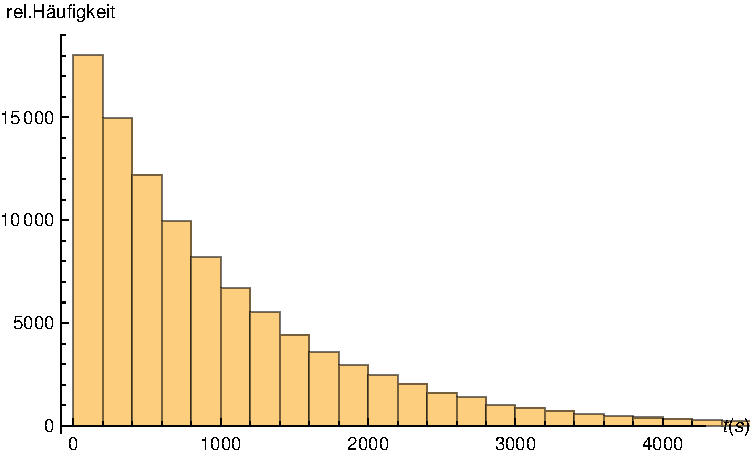
\includegraphics[width=0.8\textwidth]{abbildungen/distribution/histogramm.pdf}
		\caption{Histogramm der generierten Zufallszahlen}
		\label{fig:Histogramm}
	\end{minipage}%
	\begin{minipage}{0.5\textwidth}
		\centering
		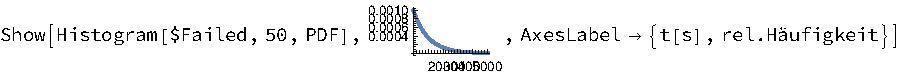
\includegraphics[width=0.8\textwidth]{abbildungen/distribution/histogrammExpVerteilung.pdf}
		\caption{Histogramm einer Exponentialverteilung}
		\label{fig:HistogrammExp}
	\end{minipage}
\end{figure}

Abbildung \ref{fig:Histogramm} zeigt die von der Simulation generierten Zufallszahlen in einem Histogramm. Zum besseren Vergleich zeigt Abbildung \ref{fig:HistogrammExp} das Histogramm einer Exponentialverteilung. Beide Abbildungen weisen einen nahezu identischen Verlauf auf, was ein Indiz für eine Exponentialverteilung der Daten darstellt.

\begin{figure}[htpb]
	\centering
	\includegraphics[width=0.8\textwidth]{abbildungen/distribution/quantilePlot.pdf}
	\caption{Quantil-Quantil-Diagramm der generierten Zufallszahlen}
	\label{fig:QQPlot}
\end{figure}

In Abbildung \ref{fig:QQPlot} werden die generierten Zufallszahlen in einem Quantil-Quantil-Diagramm dargestellt. Die blaue, gestrichelte Ursprungsgerade zeigt den Verlauf einer Exponentialverteilung im Quantil-Quantil-Diagramm. Die generierten Daten werden durch die blaue Linie repräsentiert. Die Abbildung zeigt somit, dass beide Linien nahezu deckungsgleich sind und es nur eine sehr geringe Abweichung gibt. Das Quantil-Quantil-Diagramm liefert somit einen weiteres Indiz dahingehend, dass die generierten Zufallszahlen tatsächlich exponentialverteilt sind.

\subsection{Rechnerische Überprüfung}
Für eine weitere Überprüfung werden die generierten Daten mittels Shapiro-Wilk-, Cramér-von-Mises- und Anderson-Darling-Test auf eine Exponentialverteilung überprüft. Die Hypothese H0 lautet hierbei: \\
$H_0:$ Die generierten Zufallszahlen sind exponentialverteilt, Signifikanzniveau $\alpha =0,05$ Die Ergebnisse der einzelnen Tests sind in der folgenden Tabelle aufgelistet: 
\[\begin{array}{l|ll}
 \text{} & \text{Statistic} & \text{P-Value} \\
\hline
 \text{Anderson-Darling} & 0.482866 & 0.764349 \\
 \text{Cram{\' e}r-von Mises} & 0.0690154 & 0.757621 \\
 \text{Kolmogorov-Smirnov} & 0.00201837 & 0.80994 \\
 \text{Kuiper} & 0.00390365 & 0.478494 \\
 \text{Pearson }\chi ^2 & 191.088 & 0.643726 \\
 \text{Watson }U^2 & 0.0689189 & 0.503982 \\
\end{array}\]


\\
Laut dem Shapiro-Wilk-Test kann die Nullhypothese nicht abgelehnt werden, da der p-Wert mit $0,80994$ deutlich über dem Signifikanzniveau von $0,05$ liegt. Ebenso kann die Nullhypothese bei den Cramér-von-Mises- und Anderson-Darling-Tests nicht abgelehnt werden, da der p-Wert hier ebenso mit $0,764349$ bzw. $0,0764349$ deutlich über dem Signifikanznievau liegt.\\
Durch die Tests kann somit eine Exponentialverteilung der generierten Zufallszahlen nicht wiederlegt werden. In Kombination mit der graphischen Überprüfung ist es plausibel, wenn von exponentialverteilten Werten ausgegangen wird. Ein entgültiger Beweis kann nicht erbracht werden.

\section{Auswertung der Ergebnisse}
Im Zuge dieses Kapitels werden alle Ergebnisse der Simulation und die daraus errechneten Werte erläutert. Zusätzlich werden relevante Größen durch Plots veranschaulicht. Die einzelnen Auswertungen werden mit Hilfe des Theorems von Little validiert.

\subsection{Modell \glqq Ein Telefon\grqq} 
Für den in Kapitel \ref{sec:Requirements} REFERENZAUFANFORDERUNG aufgelisteten ersten Betriebsmodus (ein Server, welcher alle Clients bedient) werden im folgenden die Auswertungen aufgeführt. Exemplarisch werden vier verschiedene durchschnittliche Ankunftszeiten für die Clients verwendet. Zunächst wird eine durchschnittliche Ankunftszeit von $1000s$ angenommen, was bei einer durchschnittlichen Telefonierdauer von $100s$ (Dauer der Serverbelegung) einer sehr geringen Serverauslastung entspricht. Anschließend werden mit den durchschnittlichen Ankunftszeiten von $800s$, $400s$ und $100s$ die Auswirkungen von höherer Serverauslastung auf das Ergebnis der Simulation erläutert. \\

Für jede durchschnittliche Ankunftszeit werden zunächst die zu erwartenden Werte, basierend auf den Formeln für M/M/1 Warteschlangenmodelle ermittelt. Die einzelnen Formeln sind im folgenden Kapitel aufgeführt. Betrachtet werden hierbei, wie in den \ref{sec:Requirements} erläutert die durchschnittliche Anzahl von Kunden im System, durchschnittliche Warteschlangenlänge, durchschnittliche Verweildauer im System und die durchschnittliche Verweildauer in der Warteschlange. Die berechneten Größen werden als Erwartungswerte betrachtet gegen die die durch die Simulation ermittelten Werte geprüft werden. 

Die Maßnahmen für die Verifikation der implementierten Simulation werden im Kapitel (REFERENZ AUF DIE UNITTEST KAPITEL) näher beschrieben. In den folgenden Abbildungen wird die durchschnittliche Zwischenankunftszeit mit \glqq MeanAr\grqq abgekürzt.

\subsubsection{Formeln für M/M/1 Warteschlangenmodelle}
\label{Formeln}
Die im folgenden aufgeführten Formeln gelten für M/M/1 Warteschlangenmodelle. Mit $Ls$ wird die durchschnittliche Anzahl von Kunden im System bezeichnet. $Lq$ gibt die durchschnittliche Länge der Warteschlange an. $Ws$ definiert die durchschnittliche Verweildauer der einzelnen Kunden im System und $Wq$ die durchschnittliche Verweildauer in der Warteschlange. 

\begin{equation}
Ls=\frac{\lambda}{\mu - \lambda}
\end{equation}
\begin{equation}
Lq=\frac{\rho\lambda}{\mu - \lambda}
\end{equation}
\begin{equation}
Ws=\frac{1}{\mu - \lambda}
\end{equation}
\begin{equation}
Wq=\frac{\rho}{\mu - \lambda}
\end{equation}

In den einzelnen Gleichungen sind $\lambda$, $\mu$ und $\rho$ wie folgt definiert: $\lambda$ beschreibt die durchschnittliche Ankunftszeit der Kunden pro Sekunde. $\mu$ definiert die durchschnittliche Telefonierdauer der Kunden pro Sekunde. Und $\rho$ beschreibt die durchschnittliche Auslastung des Telefons. 

\begin{equation}
\rho=\frac{\lambda}{\mu}
\end{equation}

Quelle: $http://www.business.uzh.ch/dam/jcr:00000000-0451-792f-ffff-fffffe13aac9/ServiceManagement_Warteschlangenmodelle.pdf$

\subsubsection{Validierung der einzelnen Auswertung auf Basis des Little Theorems}
Laut dem Theorem von Little muss die durchschnittliche Anzahl von Kunden in einem Warteschlangensystem gleich dem Produkt aus der durchschnittlichen Ankunftsrate ($\Lambda$) und der durchschnittlichen Verweildauer ($Ws$) im System sein, wenn das System sich in einem eingeschwungenen Zustand befindet.

\begin{equation}
Ls=\lambda*Ws
\end{equation}

Stellt man die Formel um, muss im eingeschwungenen Zustand gelten:

\begin{equation}
\label{eq:little}
\lambda*Ws - Ls=0
\end{equation}

Anhand dieser Gleichung werden im weiteren Verlauf der Studienarbeit die einzelnen Auswertungen validiert.

\subsubsection{Durchschnittliche Zwischenankunftszeit der Clients: $1000s$}

\paragraph{Theoretische Erwartungswerte laut M/M/1 Warteschlangenmodell}
\\
Bei einer durchschnittlichen Zwischenankunftszeit von $1000s$ ($\lambda=\frac{1}{1000}$, $\mu=\frac{1}{100}$)ergeben sich, basierend auf den in Abschnitt \ref{Formeln} aufgeführten Formeln, folgende Erwartungswerte:
\begin{equation}
Ls=0,111111
\end{equation}
\begin{equation}
Lq=0,0111111
\end{equation}
\begin{equation}
Ws=111,111
\end{equation}
\begin{equation}
Wq=11,1111
\end{equation}
Die einzelnen Erwartungswerte sind in den nachfolgenden Abbildungen durch eine gelbe Linie hervorgehoben.

\paragraph{Verwendung der implementierten Java-Simulation, Berechnung in Java}
\label{JavaOnePhone1000}
\\
\begin{figure}[htpb]
	\centering
	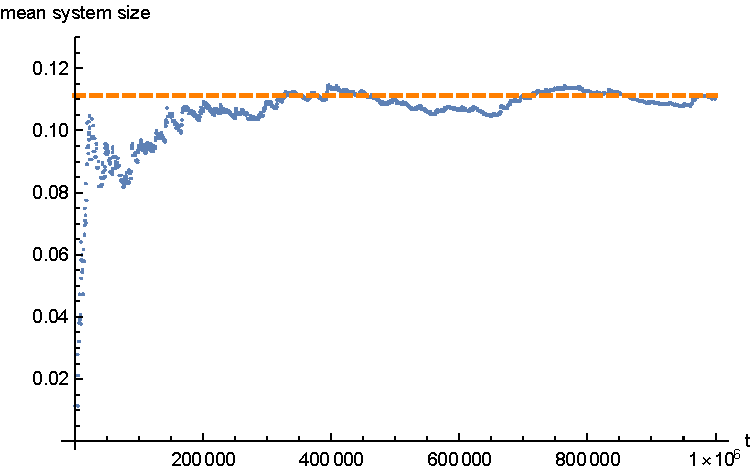
\includegraphics[width=0.8\textwidth]{abbildungen/1_Phone/Arrival_1000_Serve_100_dur_1000000_Skip_0/MeanSystemSize.pdf}
	\caption{Durchschnittliche Anzahl an Kunden im System, MeanAr = $1000s$}
	\label{fig:meanSystemSize1000}
\end{figure}

Abbildung \ref{fig:meanSystemSize1000} zeigt die durchschnittliche Anzahl an Kunden im System an. Ab einer Simulationszeit von ca $200000s$ liegt diese durchschnittlich bei $0.11$, schwankt jedoch bis zum Ende der Simulation um ca. $0,01$. Der Erwartungswert von $0,111111$ wird durch die Simulation nicht exakt erreicht. Es muss von einem systematischen Fehler von ca. $0,01$ ausgegangen werden. Weitere Erkenntnisse liefert die Validierung mit Hilfe des Little Theorems. Allgemein zeigt dieser Plot, dass die durchschnittliche Anzahl an Kunden im System sehr gering ist. Durch die Vergleichsweise kurze Telefonierzeit in Kombination mit einer lange Zwischenankunftszeit ist dieser Wert plausibel.

\begin{figure}[htpb]
	\centering
	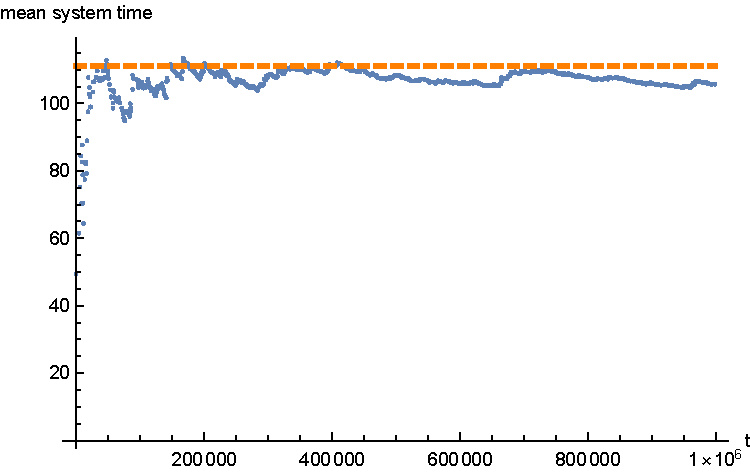
\includegraphics[width=0.8\textwidth]{abbildungen/1_Phone/Arrival_1000_Serve_100_dur_1000000_Skip_0/MeanSystemTime.pdf}
	\caption{Durchschnittliche Verweildauer der Kunden im System, MeanAr = $1000s$}
	\label{fig:meanSystemTime1000}
\end{figure}

Betrachtet man Abbildung \ref{fig:meanSystemTime1000}, wird deutlich, dass die durchschnittliche Verweilsdauer im System bis zu einer Simulationszeit von $200000s$ stark variiert. Doch auch mit steigender Simulationszeit bleibt sie unter dem erwarteten Wert von $111.111$ bei durchschnittlich. Der Grund hierfür könnte wiederum ein systematischer Fehler in der Berechnung, beispielsweise aufgrund von Ungenauigkeiten durch Runden sein.

\begin{figure}[htpb]
	\centering
	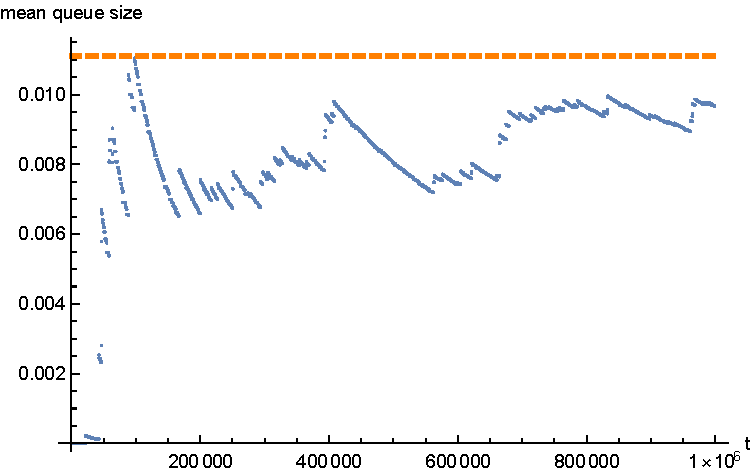
\includegraphics[width=0.8\textwidth]{abbildungen/1_Phone/Arrival_1000_Serve_100_dur_1000000_Skip_0/MeanQueueSize.pdf}
	\caption{Durchschnittliche Warteschlangenlänge, MeanAr = $1000s$}
	\label{fig:meanQueueSize1000}
\end{figure}

Bei der Betrachtung der in Abbildung \ref{fig:meanQueueSize1000} gezeigte durchschnittliche Warteschlangenlänge fällt auf, dass die Werte wiederum bis zu einer Simulationsdauer von $200000s$ stark variieren schwanken. Anschließend nähern sich die Werte dem dem Erwartungswert von $0,0111111$ an, bleiben jedoch unterhalb. Es ist hierbei wiederum von einem systematischen Fehler von ca. $0,0015$ auszugehen.

\begin{figure}[htpb]
	\centering
	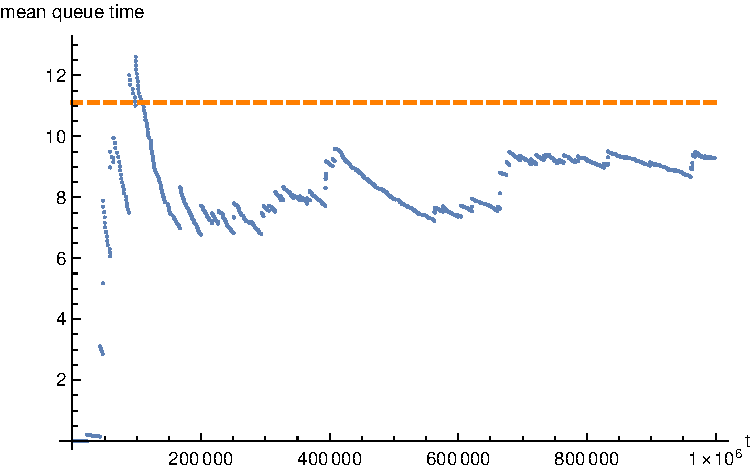
\includegraphics[width=0.8\textwidth]{abbildungen/1_Phone/Arrival_1000_Serve_100_dur_1000000_Skip_0/MeanQueueTime.pdf}
	\caption{Durchschnittliche Verweildauer in der Warteschlange , MeanAr = $1000s$}
	\label{fig:meanQueueTime1000}
\end{figure} 

Die in Abbildung \ref{fig:meanQueueTime1000} aufgeführte durchschnittliche Verweildauer in der Warteschlange weißt einen ähnlichen Verlauf auf wie die in Abbildung \ref{fig:meanQueueSize1000} gezeigte durchschnittliche Warteschlangenlänge. Dieses Verhalten ist plausibel, da bei einer größeren Warteschlangenlänge auch die Wartezeit in der Warteschlange steigt. Gegen Ende der Simulation näher sich die durchschnittliche Verweildauer in der Warteschlange dem Erwartungswert von $11,1111$ an, bleibt jedoch mit einer Abweichung von ca. $1,51$ unterhalb.

\begin{figure}[htpb]
	\centering
	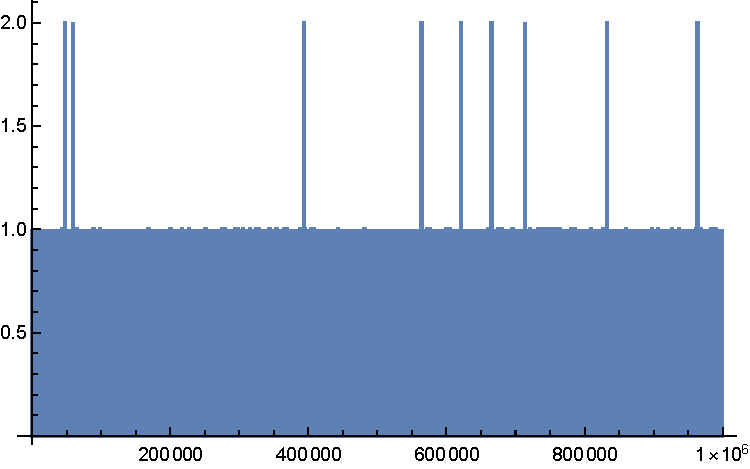
\includegraphics[width=0.8\textwidth]{abbildungen/1_Phone/Arrival_1000_Serve_100_dur_1000000_Skip_0/QueueStepPlotAll.pdf}
	\caption{Warteschlangenlänge (ungefiltert) , MeanAr = $1000s$}
	\label{fig:QueueStepPlotAll1000}
\end{figure} 
\begin{figure}[htpb]
	\centering
	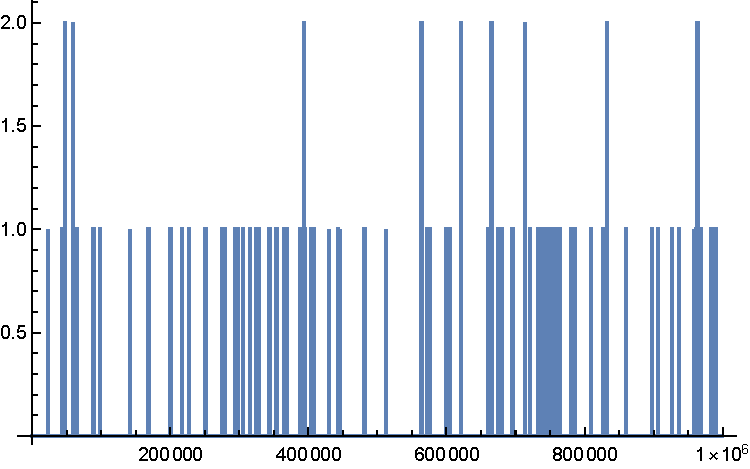
\includegraphics[width=0.8\textwidth]{abbildungen/1_Phone/Arrival_1000_Serve_100_dur_1000000_Skip_0/QueueStepPlotAllFiltered.pdf}
	\caption{Warteschlangenlänge (gefiltert) , MeanAr = $1000s$}
	\label{fig:QueueStepPlotAllFiltered1000}
\end{figure} 

Die Abbildung \ref{fig:QueueStepPlotAll1000} zeigt die einzelnen Werte für die Warteschlangenlänge über die Simulationszeit. Diese Abbildung ist nicht aussagekräftig. Hintergrund dafür ist die Implementierung der Simulation. Im Warteschlangenmodell wird zwischen drei verschiedenen Events unterschieden. Betritt ein neuer Kunde den Telefonshop, wird ein Arrival Event ausgelöst und die Warteschlangenlänge wird um 1 erhöht. Ist das Telefon frei, wird ein Begin Event ausgelöst und die Warteschlangenlänge wird um 1 reduziert. Hat ein Kunde sein Telefonat beendet, wird ein Finish Event ausgelöst, was wiederum ein Begin Event auslöst, da das Telefon frei ist. Ein Problem gibt es hierbei für den Fall, dass kein Kunde im Laden steht und somit auch die Warteschlange leer und das Telefon frei ist. Betritt nun ein neuer Kunde den Laden, wird ein Arrival Event ausgelöst und direkt anschließend ein Begin Event, da das Telefon frei ist und der Kunde sein Telefonat sofort beginnen kann. Er befindet sich somit für $0s$ in der Warteschlange. Aufgrund der Events wird die Warteschlangenlänge jedoch trotzdem erhöht und direkt wieder gesenkt. Es gibt somit für den gleichen Zeitstempel zwei unterschiedliche Warteschlangenlängen. Abbildung \ref{fig:QueueStepPlotAllFiltered1000} zeigt die gleiche Situation ohne die eben erläuterte Situation. Es wird hierbei nur eine Warteschlangenlänge angezeigt, wenn auch wirklich ein Kunde länger als $0s$ in der Warteschlange wartet. Da das System nur sehr gering ausgelastet ist, ist die geringe Warteschlangenlänge plausibel.\\
Abschließend sind im folgenden die von der implementierten Simulation berechneten Werte für die durchschnittliche Warteschlangenlänge, Wartezeit in der Warteschlange, Anzahl an Clients im System und Zeit im System aufgeführt:
%\[\begin{array}{cc}
 \text{mean queue size} & 0.00537307572764891636692565082375430880024384373 \\
 \text{mean queue time} & 8.19291 \\
 \text{mean system size} & 0.06921258430823697932263116253494454280311475015 \\
 \text{mean system time} & 105.458 \\
\end{array}\]


FEHLT !!!!!!!!!!!!!!!!!!!!!!!!!!!!!

\paragraph{Validierung der Simulation}
\\
\begin{figure}[htpb]
	\centering
	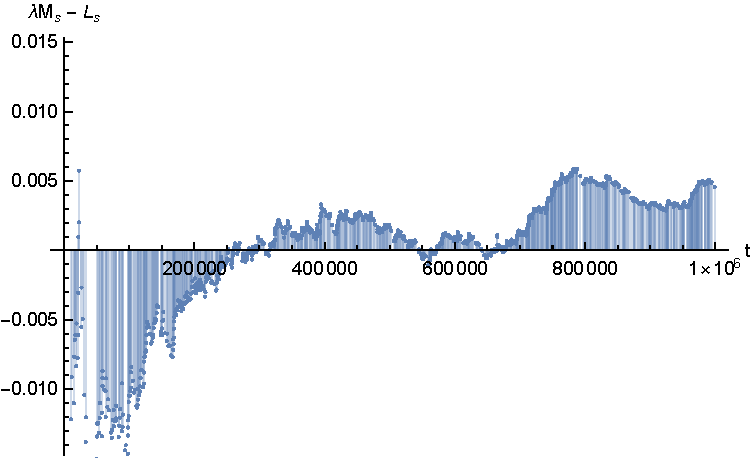
\includegraphics[width=0.8\textwidth]{abbildungen/1_Phone/Arrival_1000_Serve_100_dur_1000000_Skip_0/LittleSystem.pdf}
	\caption{Darstellung der Differenz: $\lambda * Ws - Ls$ über die Simulationszeit (Little Theorem)}
	\label{fig:LittleSystem1000}
\end{figure} 

In Abbildung \ref{fig:LittleSystem1000} ist der Verlauf der Gleichung \ref{eq:little} über die Simulationszeit aufgeführt. Ab einer Simulationsdauer von ca. $350000s$ liegt der Wert sehr nach an dem geforderten Erwartungswert von $0$, schwankt jedoch bis zum Ende der Simulation im Bereich von $0,004$. Da die Differenz zum Erwartungswert sehr gering ist, liegt die Ursache für diese Abweichung vermutlich in Ungenauigkeiten bei der Berechung der Werte. Die durchschnittliche Anzahl an Kunden im System wird entweder um $0,004$ zu gering angenommen, oder die Verweildauer der Kunden im System um $0,004$ zu lang. Ebenso ist eine Kombination der beiden Fehler möglich. Insgesamt deckt sich diese Aussage mit den Abweichungen in den einzelnen Abbildungen.

\subsubsection{Durchschnittliche Zwischenankunftszeit der Clients: $400s$}
\paragraph{Theoretische Erwartungswerte laut M/M/1 Warteschlangenmodell}
\\
Bei einer durchschnittlichen Zwischenankunftszeit von $400s$ ($\lambda=\frac{1}{400}$, $\mu=\frac{1}{100}$)ergeben sich, basierend auf den in Abschnitt \ref{Formeln} aufgeführten Formeln, folgende Erwartungswerte:
\begin{equation}
Ls=0,333333
\end{equation}
\begin{equation}
Lq=0,0833333
\end{equation}
\begin{equation}
Ws=133,333
\end{equation}
\begin{equation}
Wq=33,3333
\end{equation}
Die einzelnen Erwartungswerte sind in den nachfolgenden Abbildungen durch eine gelbe Linie hervorgehoben.

\paragraph{Verwendung der implementierten Java-Simulation, Berechnung in Java}
\\
\begin{figure}[htpb]
	\centering
	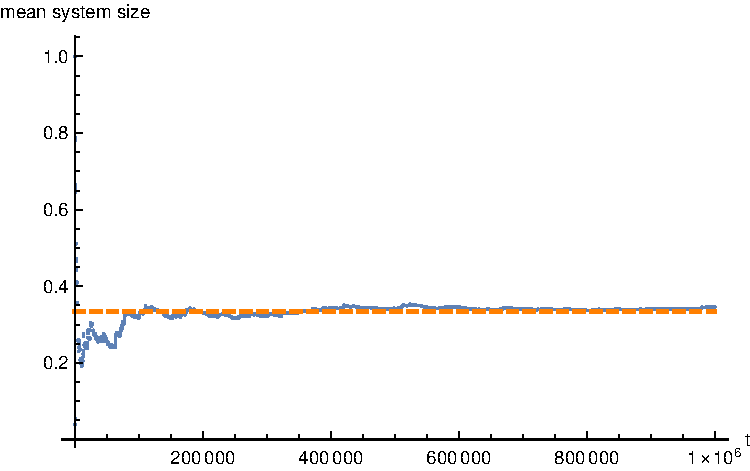
\includegraphics[width=0.8\textwidth]{abbildungen/1_Phone/Arrival_400_Serve_100_dur_1000000_Skip_0/MeanSystemSize.pdf}
	\caption{Durchschnittliche Anzahl an Kunden im System, MeanAr = $400s$}
	\label{fig:meanSystemSize400}
\end{figure}

Abbildung \ref{fig:meanSystemSize400} zeigt die durchschnittliche Anzahl an Kunden im System an. Ab einer Simulationszeit von ca $400000s$ schwankt diese nur noch sehr gering, liegt jedoch über dem Erwartungswert von $0,333333$. Es ist von einem systematischen Fehler von $0,01$ auszugehen.

\begin{figure}[htpb]
	\centering
	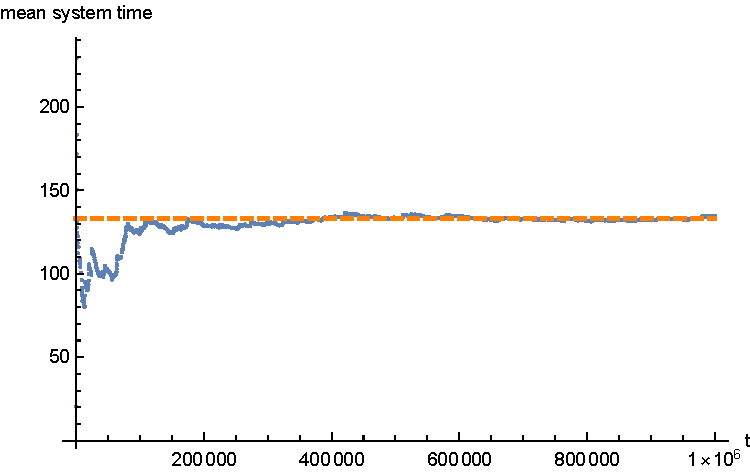
\includegraphics[width=0.8\textwidth]{abbildungen/1_Phone/Arrival_400_Serve_100_dur_1000000_Skip_0/MeanSystemTime.pdf}
	\caption{Durchschnittliche Verweildauer der Kunden im System, MeanAr = $400s$}
	\label{fig:meanSystemTime400}
\end{figure}

Auch die in Abbildung \ref{fig:meanSystemTime400} dargestellte durchschnittliche Verweildauer im System schwankt bis zu einer Simulationsdauer von ca. $400000s$ stark. Anschließend schwankt sie um ca. $2$ um den erwarteten Wert von $133,333$.

\begin{figure}[htpb]
	\centering
	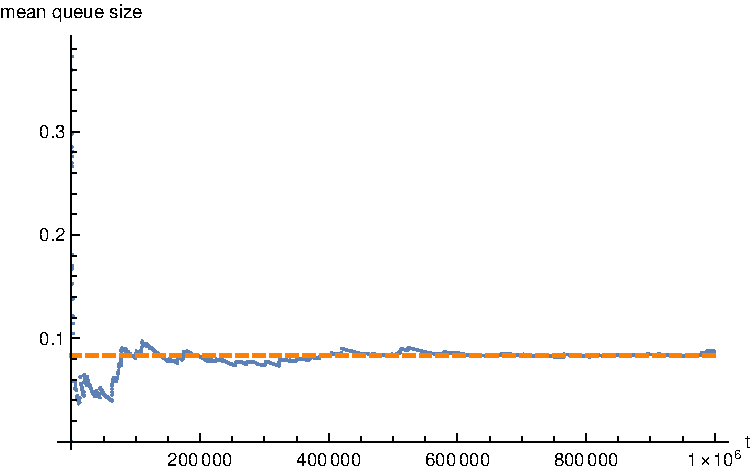
\includegraphics[width=0.8\textwidth]{abbildungen/1_Phone/Arrival_400_Serve_100_dur_1000000_Skip_0/MeanQueueSize.pdf}
	\caption{Durchschnittliche Warteschlangenlänge, MeanAr = $400s$}
	\label{fig:meanQueueSize400}
\end{figure}

Die in Abbildung \ref{fig:meanQueueSize400} gezeigte durchschnittliche Warteschlangenlänge schwankt ebenso ab einer Simulationsdauer von ca. $400000s$ nur noch um ca. $0,001$ um den erwarteten Wert von $0,0833333$.

\begin{figure}[htpb]
	\centering
	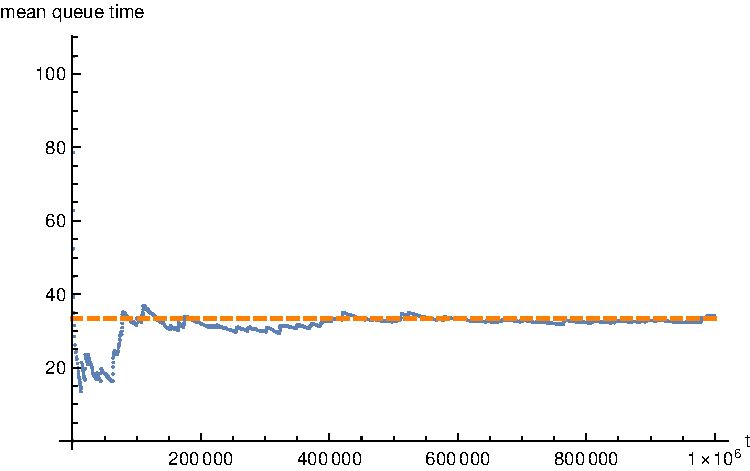
\includegraphics[width=0.8\textwidth]{abbildungen/1_Phone/Arrival_400_Serve_100_dur_1000000_Skip_0/MeanQueueTime.pdf}
	\caption{Durchschnittliche Verweildauer in der Warteschlange , MeanAr = $400s$}
	\label{fig:meanQueueTime400}
\end{figure} 

Die in Abbildung \ref{fig:meanQueueTime400} aufgeführte durchschnittliche Verweildauer in der Warteschlange weißt einen ähnlichen Verlauf auf wie die in Abbildung \ref{fig:meanQueueSize400} gezeigte durchschnittliche Warteschlangenlänge. Dieses Verhalten ist plausibel, da bei einer größeren Warteschlangenlänge auch die Wartezeit in der Warteschlange steigt. Beide Werte schwanken ab einer Simulationsdauer von ca. $400000s$ um den Erwartungswert. Die durchschnittliche Verweildauer in der Warteschlange schwankt um ca. $2$ um den Erwartungswert von $33,3333$. 

Im der folgenden Tabelle sind die von der implementierten Simulation berechneten Werte für die durchschnittliche Warteschlangenlänge, Wartezeit in der Warteschlange, Anzahl an Clients im System und Zeit im System aufgeführt:
%\[\begin{array}{cc}
 \text{mean queue size} & 0.00537307572764891636692565082375430880024384373 \\
 \text{mean queue time} & 8.19291 \\
 \text{mean system size} & 0.06921258430823697932263116253494454280311475015 \\
 \text{mean system time} & 105.458 \\
\end{array}\]


FEHLT !!!!!!!!!!!!!!!!!!!!!!!!!!!!!

\begin{figure}[htpb]
	\centering
	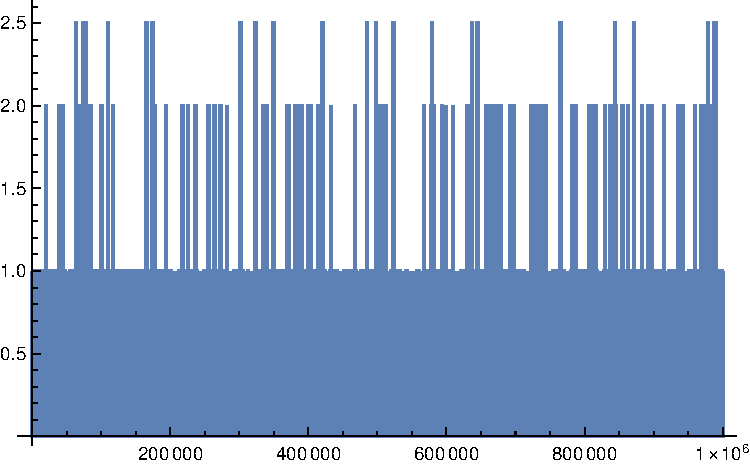
\includegraphics[width=0.8\textwidth]{abbildungen/1_Phone/Arrival_400_Serve_100_dur_1000000_Skip_0/QueueStepPlotAll.pdf}
	\caption{Warteschlangenlänge (ungefiltert) , MeanAr = $400s$}
	\label{fig:QueueStepPlotAll400}
\end{figure} 
\begin{figure}[htpb]
	\centering
	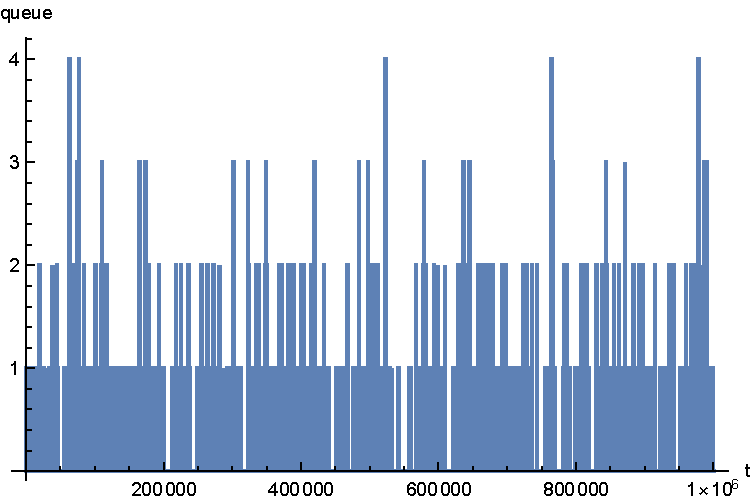
\includegraphics[width=0.8\textwidth]{abbildungen/1_Phone/Arrival_400_Serve_100_dur_1000000_Skip_0/QueueStepPlotAllFiltered.pdf}
	\caption{Warteschlangenlänge (gefiltert) , MeanAr = $400s$}
	\label{fig:QueueStepPlotAllFiltered400}
\end{figure}

Abschließend sind in den Abbildungen \ref{fig:QueueStepPlotAll400} und \ref{fig:QueueStepPlotAllFiltered400} jeweils die Länge der Warteschlange dargestellt. Aufgrund des in \ref{JavaOnePhone1000} erläuterten Problems mit der Inkrementierung bzw. Dekrementierung der Warteschlangenlänge bei den einzelnen Events, ist die tatsächliche Länge in der Abbildung \ref{fig:QueueStepPlotAllFiltered400} gefiltert besser zu sehen. Die Warteschlangenlänge ist größer als bei einer durchschnittlichen Zwischenankunftszeit von $1000s$, doch das Telefon ist noch nicht zu voll ausgelastet, da die Warteschlangenlänge phasenweise noch immer $0$ ist.


\paragraph{Validierung der Simulation}
\\
\begin{figure}[htpb]
	\centering
	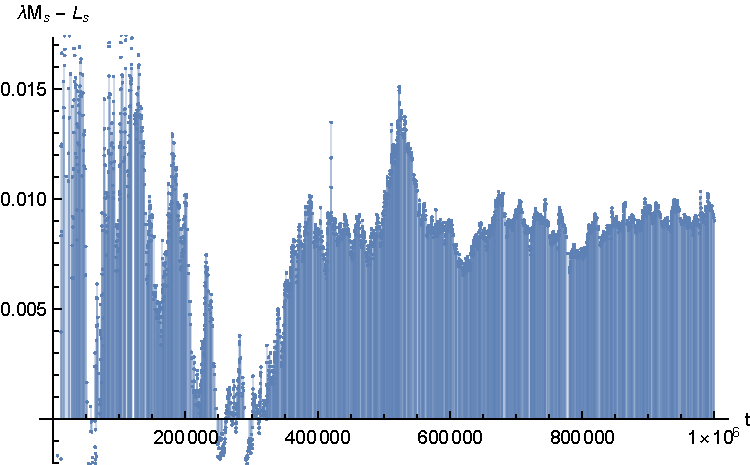
\includegraphics[width=0.8\textwidth]{abbildungen/1_Phone/Arrival_400_Serve_100_dur_1000000_Skip_0/LittleSystem.pdf}
	\caption{Darstellung der Differenz: $\lambda * Ws - Ls$ über die Simulationszeit (Little Theorem)}
	\label{fig:LittleSystem400}
\end{figure}

In Abbildung \ref{fig:LittleSystem400} ist der Verlauf der Gleichung \ref{eq:little} über die Simulationszeit aufgeführt. Ab einer Simulationsdauer von ca. $400000s$ schwankt der Wert nur noch geringfügig. Die Werte liegen jedoch bis zum Ende der Simulation bei durchschnittlich ca. $0,009$. Wie auch bei der Auswertung der Simulation mit einer durchschnittlichen Zwischenankunftszeit von $1000s$, kann hier wiederum von einem systematischen Fehler von $0,009$ mit den selben Ursachen ausgegangen werden. Die Abweichung ist hier größer, da aufgrund der niedrigeren Zwischenankunftszeit deutlich mehr Kunden den Laden besucht haben und somit mehr Zeiten verrechnet wurden. Insgesamt deckt sich dieser Fehler mit den Abweichungen in den einzelnen Abbildungen.

\subsubsection{Durchschnittliche Ankunftszeit der Clients: $100s$}
\paragraph{Theoretische Erwartungswerte laut M/M/1 Warteschlangenmodell}
\\
Für durchschnittliche Zwischenankunftszeit und durchschnittliche Telefonierdauer $100s$ ($\lambda=\frac{1}{100}$, $\mu=\frac{1}{100}$), lassen sich die durchschnittliche Warteschlangenlänge, Wartezeit in der Warteschlange, Anzahl an Clients im System und Zeit im System nicht berechnen. Die Warteschlangenlänge steigt aufgrund der zu hohen Auslastung des Telefons gegen unendlich. Somit steigt auch die durchschnittliche Anzahl an Kunden im System gegen unendlich, da diese sich aus den Kunden in der Warteschlange und dem Kunden am Telefon zusammensetzt. Bei einer unendlich langen Warteschlange ist folglich auch die Wartezeit unendlich lang. Außerdem folgt aus einer unendlichen Anzahl von Kunden im System auch, dass die durchschnittliche Zeit im System unendlich lang wird.

\paragraph{Verwendung der implementierten Java-Simulation, Berechnung in Java}

\begin{figure}[htpb]
	\centering
	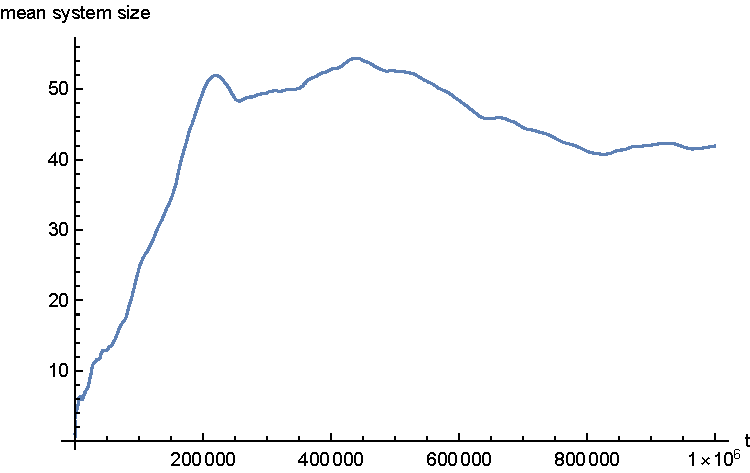
\includegraphics[width=0.8\textwidth]{abbildungen/1_Phone/Arrival_100_Serve_100_dur_1000000_Skip_0/MeanSystemSize.pdf}
	\caption{Durchschnittliche Anzahl an Kunden im System, MeanAr = $100s$}
	\label{fig:meanSystemSize100}
\end{figure}

Abbildung \ref{fig:meanSystemSize100} zeigt die durchschnittliche Anzahl an Kunden im System an. Durch die großen Schwankungen kann nicht von einem eingeschwungenen System ausgegangen werden. Für eine genauere Beurteilung müsste die Simulation hierfür mit einer längeren Simulationsdauer erneut durchgeführt werden. Ob die durchschnittliche Anzahl der Kunden an Kunden im System gegen den erwarteten Wert von unendlich steigt, kann erst dann analysiert werden.

\begin{figure}[htpb]
	\centering
	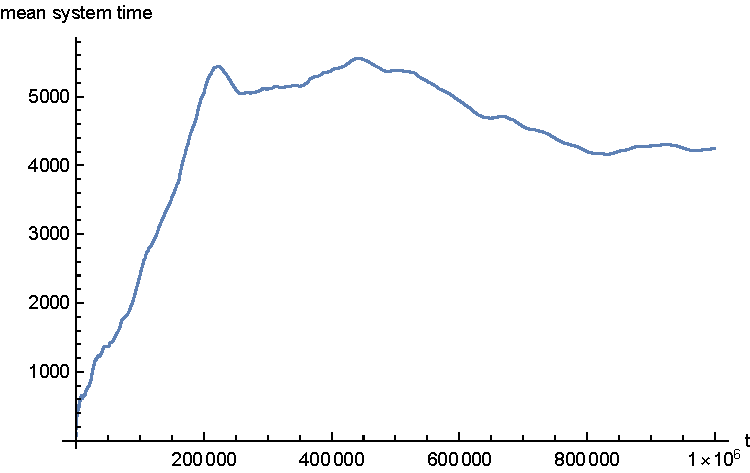
\includegraphics[width=0.8\textwidth]{abbildungen/1_Phone/Arrival_100_Serve_100_dur_1000000_Skip_0/MeanSystemTime.pdf}
	\caption{Durchschnittliche Verweildauer der Kunden im System, MeanAr = 100}
	\label{fig:meanSystemTime100}
\end{figure}

Abbildung \ref{fig:meanSystemTime100} zeigt die durchschnittliche Verweildauer der Kunden im System. Wiederum kann davon ausgegangen werden, dass das System noch nicht eingeschwungen war, bzw. nicht einschwingen wird. 

\begin{figure}[htpb]
	\centering
	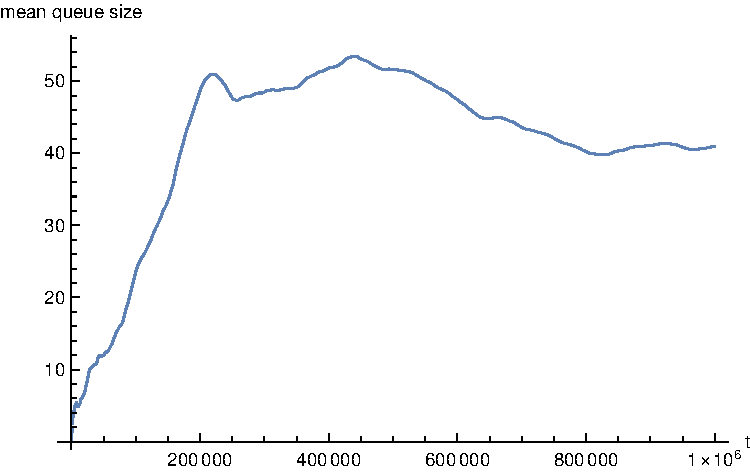
\includegraphics[width=0.8\textwidth]{abbildungen/1_Phone/Arrival_100_Serve_100_dur_1000000_Skip_0/MeanQueueSize.pdf}
	\caption{Durchschnittliche Warteschlangenlänge, MeanAr = 100}
	\label{fig:meanQueueSize100}
\end{figure}

Die Abbildungen \ref{fig:meanQueueSize100} und \ref{fig:meanQueueTime100} und auch weisen einen ähnlichen Verlauf auf wie \ref{fig:meanSystemTime100}. Die Werte schwanken ebenfalls bis zum Ende der Simulation stark.

\begin{figure}[htpb]
	\centering
	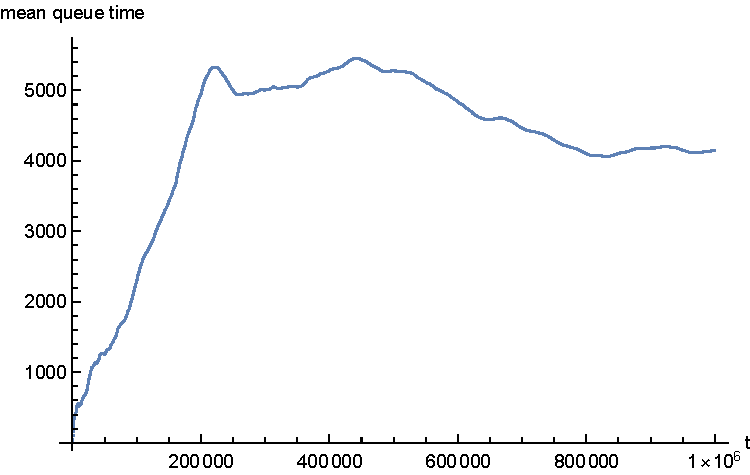
\includegraphics[width=0.8\textwidth]{abbildungen/1_Phone/Arrival_100_Serve_100_dur_1000000_Skip_0/MeanQueueTime.pdf}
	\caption{Durchschnittliche Verweildauer in der Warteschlange , MeanAr = 100}
	\label{fig:meanQueueTime100}
\end{figure} 

Abschließend sind in den Abbildungen \ref{fig:QueueStepPlotAll100} und \ref{fig:QueueStepPlotAllFiltered100} jeweils die Länge der Warteschlange dargestellt. Aufgrund des in \ref{JavaOnePhone1000} erläuterten Problems mit der Inkrementierung bzw. Dekrementierung der Warteschlangenlänge bei den einzelnen Events, zeigt Abbildung \ref{fig:QueueStepPlotAllFiltered400} wiederum die gefilterten Werte. Die Werte in beiden Abbildungen schwanken jedoch so stark, dass kein Unterschied mehr ersichtlich ist. Gegen Ende der Simulation steigen die Werte deutlich an. Ob sie gegen den erwarteten Wert von unendlich ansteigen lässt sich nur im Zuge einer erneuten Simulation mit einer längeren Simulationsdauer ermitteln.

\begin{figure}[htpb]
	\centering
	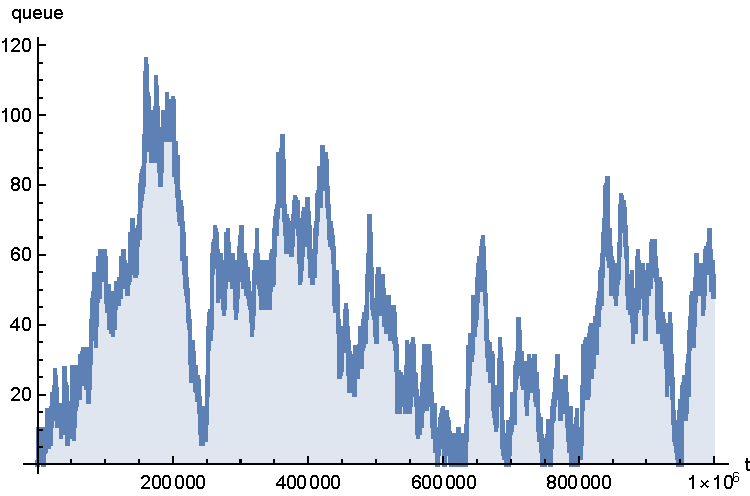
\includegraphics[width=0.8\textwidth]{abbildungen/1_Phone/Arrival_100_Serve_100_dur_1000000_Skip_0/QueueStepPlotAll.pdf}
	\caption{Warteschlangenlänge (ungefiltert) , MeanAr = 100}
	\label{fig:QueueStepPlotAll100}
\end{figure} 
\begin{figure}[htpb]
	\centering
	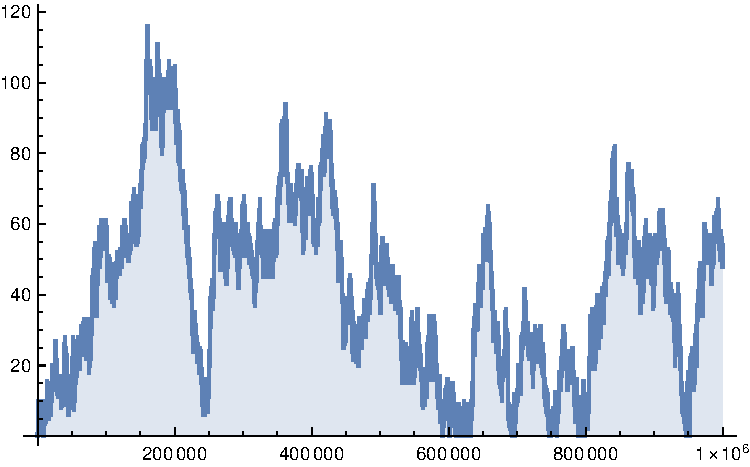
\includegraphics[width=0.8\textwidth]{abbildungen/1_Phone/Arrival_100_Serve_100_dur_1000000_Skip_0/QueueStepPlotAllFiltered.pdf}
	\caption{Warteschlangenlänge (gefiltert) , MeanAr = 100}
	\label{fig:QueueStepPlotAllFiltered100}
\end{figure} 

Abschließend sind im folgenden die von der implementierten Simulation berechneten Werte für die durchschnittliche Warteschlangenlänge, Wartezeit in der Warteschlange, Anzahl an Clients im System und Zeit im System aufgeführt:
%\[\begin{array}{cc}
 \text{mean queue size} & 0.00537307572764891636692565082375430880024384373 \\
 \text{mean queue time} & 8.19291 \\
 \text{mean system size} & 0.06921258430823697932263116253494454280311475015 \\
 \text{mean system time} & 105.458 \\
\end{array}\]


FEHLT !!!!!!!!!!!!!!!!!!!!!!!!!!!!!

\paragraph{Validierung der Simulation}
\begin{figure}[htpb]
	\centering
	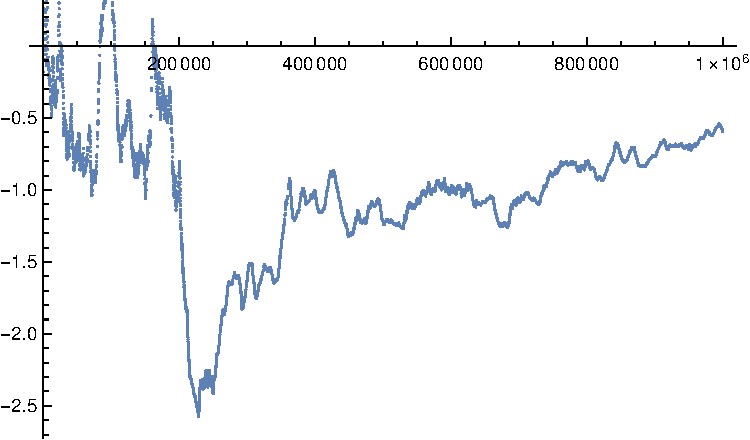
\includegraphics[width=0.8\textwidth]{abbildungen/1_Phone/Arrival_100_Serve_100_dur_1000000_Skip_0/LittleSystem.pdf}
	\caption{Darstellung der Differenz: $\lambda * Ws - Ls$ über die Simulationszeit (Little Theorem)}
	\label{fig:LittleSystem100}
\end{figure} 
In Abbildung \ref{fig:LittleSystem100} ist der Verlauf der Gleichung \ref{eq:little} über die Simulationszeit aufgeführt. Im Vergleich zu den beiden Auswertungen mit Zwischenankunftszeiten von $1000s$ bzw. $400s$ wird deutlich, dass die Abweichung vom den geforderten Wert $0$ in dieser Abbildung deutlich größer ist. Es kann somit nicht von einem eingeschwungenen System ausgegangen werden. Bis zum Ende der Simulation stimmt das implementierte Modell dadurch mit der Theorie überein, welche besagt, dass wenn die durchschnittliche Zwischenankunftszeit gleich der durchschnittlichen Bediendauer ist, das System nie einschwingen kann. Ein Beweis, dass das System auch bei einer längeren Simulationsdauer nicht einschwingen würde, kann nicht erbracht werden.

\subsection{Modell \glqq Bevorzugte VIP\grqq} 

\subsubsection{Durchschnittliche Ankunftszeit der Clients: 1000}
\subsubsection{Durchschnittliche Ankunftszeit der Clients: 400}
\subsubsection{Durchschnittliche Ankunftszeit der Clients: 100}

\subsection{Modell \glqq Zusätzliches VIP Telefon\grqq} 
\subsubsection{Durchschnittliche Ankunftszeit der Clients: 1000}
\subsubsection{Durchschnittliche Ankunftszeit der Clients: 400}
\subsubsection{Durchschnittliche Ankunftszeit der Clients: 100}

\section{Fazit}

\end{document}
